\section{INTRODUCTION}

Consider the \textit{controlled} ODE
$$
	\dot{x}(t) = f(t, x(t), u(t)) = A(t) x(t) + B(t) u(t)
$$

for $A(t) \in \R^{d \times d}$, $B(t) \in \R^{d \times m}$, $u(t) \in \R^m$ and $t \in [0, T]$ where $u \in L^\infty([0, T], \R^m)$ is the control signal.

\subsection{COST FUNCTIONAL}

Consider the terminal cost
$$
	\Phi(x) = x^T M x
$$
	
for some symmetric positive definite matrix $M \in \R^{d \times d}$, then gradient of terminal cost is $(\nabla_x \Phi)(x) = 2Mx$. Consider the running cost
$$
	L(t, x, u) = x^T Q(t) x + u^T R(t) u
$$

for some collection of symmetric positive definite matrices $\set{Q(t), R(t): t \in [0, T]}$

\subsection{THE LQR PROBLEM}

The linear quadratic regulator problem is formulated by minimizing the cost functional subject to the dynamic of the \textit{controlled} ODE described above. More precisely,
\begin{align*}
	&\min_{u \in L^\infty([0, T], \R^m)} \set*{\Phi(x(t)) + \int_0^T (x^T Q(t) x(t) + u(t)^T R(t) u(t)) dt} \\
	&\text{subject to } \dot{x}(t) = f(t, x(t), u(t)) = A(t) x(t) + B(t) u(t) \text{ and } x(0) = x_0
\end{align*}

\section{NECCESSARY CONDITION VIA PONTRYAGIN MAXIMUM PRINCIPLE (PMP)}

\subsection{HAMILTONIAN}

The Hamiltonian is of the problem is

\begin{align*}
	&H(t, x, p, u)  \\
	&= p^T f(t, x, u) - L(t, x, u) \\
	&=  p^T A(t) x + p^T B(t) u - x^T Q(t) x - u^T R(t) u
\end{align*}

where $p(t) \in \R^d$ is the costate, then then gradients of $H$ with respect to its variables are
\begin{align*}
	(\nabla_p H)(t, x, p, u) &= \nabla_p (p^T (A(t) x + B(t) u) ) = A(t) x + B(t) u \\
	(\nabla_x H)(t, x, p, u) &= \nabla_x (p^T A(t) x - x^T Q(t) x) = A(t)^T p - 2 Q(t) x \\
	(\nabla_u H)(t, x, p, u) &= \nabla_u (p^T B(t) u - u^T R(t) u) = B(t)^T p - 2 R(t) u
	\end{align*}

\subsection{STATE AND COSTATE EQUATION AND HAMILTONIAN MAXIMAL CONDITION}

If $u^*(t)$ is the optimal control, $x^*(t)$ and $p^*(t)$ are the correspond state and costate trajectory, then the state equation is

\begin{align*}
	\dot{x}^* (t) 
	&= (\nabla_p H)(t, x^*(t), p^*(t), u^*(t)) \\
	&= A(t) x^*(t) + B(t) u^*(t)
\end{align*}

subject to $x^*(0) = x_0$, the costate equation is

\begin{align*}
	\dot{p}^*(t) 
	&= - (\nabla_x H)(t, x^*(t), p^*(t), u^*(t))\\
	&= - A(t)^T p^*(t) + 2 Q(t) x^*(t)
\end{align*}

subject to $p^*(T) = - (\nabla_x \Phi)(x^*(T)) = - 2 M x^*(T)$, and Hamiltonian maximal condition is
$$
	H(t, x^*(t), p^*(t), u^*(t)) \geq H(t, x^*(t), p^*(t), u(t))
$$

for any control $u(t)$ for almost every $t \in [0, T]$

\subsection{SHOW $u^*(t) = \frac{1}{2} R^{-1}(t) B^T(t) p^*(t)$ }

If the optimal control exists, assume all functions are sufficiently smooth, the control set is closed, we have
$$
	(\nabla_u H)(t, x^*(t), p^*(t), u^*(t)) = B(t)^T p^*(t) - 2 R(t) u^*(t) = 0
$$

for all $t \in [0, T]$. Since $R(t)$ is symmetric positive definite, $u^*(t) = \frac{1}{2} R^{-1}(t) B^T(t) p^*(t)$.

We can assume that $x^*(t) \neq 0$ at all time $t \in [0, T]$. Then, there exists a linear map, namely $L(t): \R^d \to \R^d$ so that $p^*(t) = L(t) x^*(t)$. Since both $x^*$ and $p^*$ are sufficiently smooth function, there exists a sufficiently function $L: [0, T] \to M_d[\R]$ where $M_d[\R]$ denotes the space of $d \times d$ matrices over $\R$

\section{LINEAR RELATIONSHIP OF $p^*(t)$ ON $x^*(t)$}

From now on, all functions are over variable $t$, we will drop \footnote{sorry, I have difficulties reading too many $(t)$s and $*s$} the notation $A(t), x^*(t)$ and simply write it as $A, x$

Set $p = -2Px$ for some $P: [0, T] \to M_d[\R]$. Then
$$
	\dot{p} = - 2 \dot{P} x - 2 P \dot{x}
$$

\subsection{RICATTI DIFFERENTIAL EQUATION (RDE)}

Recall state and costate equation
\begin{align*}
	\dot{x} &= Ax + Bu \\
	\dot{p} &= -A^T p + 2Qx
\end{align*}

subject to $x(0) = x_0$, $p(T) = -2Mx(T)$. Substitute $u = \frac{1}{2} R^{-1} B^T p$, we have

\begin{align*}
	\dot{x} &= Ax + \frac{1}{2} B R^{-1} B^T p \\
	\dot{p} &= -A^T p + 2Qx
\end{align*}


Substitute $p = -2Px$, and $\dot{p} = - 2 \dot{P} x - 2 P \dot{x}$, we have
\begin{align*}
	\dot{x} &= Ax - B R^{-1} B^T Px \\
	- 2 \dot{P} x - 2 P \dot{x} &= 2 A^T Px + 2Qx
\end{align*}

That induces an equation
$$
	- 2 \dot{P} x - 2 P (Ax - B R^{-1} B^T Px) = 2 A^T Px + 2Qx
$$

which simplifies into

$$
	(- P A - A^T P - Q +  P B R^{-1} B^T P  - \dot{P}) x = 0
$$

We can assume that $x(t)$ spans the whole $\R^d$, so
$$
	- P A - A^T P - Q +  P B R^{-1} B^T P = \dot{P}
$$

subject to $p(T) = -2Mx(T) \iff P(T) = M$

\subsection{IF $P := -\frac{1}{2} Y X^{-1} $ THEN $P$ SATISFIES RDE}

Let $X, Y: [0, T] \to M_d[\R]$ satisfying
$$
	\frac{d}{dt} \begin{bmatrix}
		X \\
		Y
	\end{bmatrix} = \begin{bmatrix}
		A & \frac{1}{2} B R^{-1} B^T \\
		2Q & -A^T
	\end{bmatrix} \begin{bmatrix}
		X \\
		Y
	\end{bmatrix} 
	\text{ and } \begin{bmatrix}
		X(T) \\
		Y(T)
	\end{bmatrix} = \begin{bmatrix}
		I \\
		-2M
	\end{bmatrix}
$$

That is equivalent to the system of equations
\begin{align*}
	\dot{X} &= AX + \frac{1}{2} B R^{-1} B^T Y \\
	\dot{Y} &= 2QX - A^T Y
\end{align*}

We assume that $X$ is invertible for all $t \in [0, T]$. Let $P = - \frac{1}{2} Y X^{-1}$, then $PX = - \frac{1}{2} Y$, differentiate both sides
$$
	\dot{P} X + P \dot{X} = - \frac{1}{2} \dot{Y}
$$

So
\begin{align*}
	\dot{P} 
	&= - \frac{1}{2} \dot{Y} X^{-1} - P \dot{X} X^{-1} \\
	&= - \frac{1}{2} (2QX - A^T Y) X^{-1} - P \tuple*{AX + \frac{1}{2} B R^{-1} B^T Y} X^{-1} \\
	&= - Q + \frac{1}{2} A^T Y X^{-1} - P A - \frac{1}{2} PBR^{-1} B^T Y X^{-1} \\
	&= - Q - A^T P - PA  + PBR^{-1} B^T P
\end{align*}

Moreover, $P(T) = - \frac{1}{2} Y(T) X(T)^{-1} = M$ which is precisely the description for RDE problem, so any $X, Y$ satisfies the above equations also solve RDE.

\section{HAMILTON-JACOBI-BELLMAN FRAMEWORK}

\subsection{HAMILTON-JACOBI-BELLMAN EQUATION}

For any $s, \tau \in [0, T]$ with $s \leq \tau$ and some $z \in \R^d$, let $V(s, z)$ be the optimal cost travelling from the state $(t, x) = (s, z)$, more precisely,

$$
	V(s, z) = \inf_u \set*{\int_s^\tau L(t, x(t), u(t)) dt + V(\tau, x(\tau))}
$$

where $x$ solves the ODE $\dot{x}(t) = f(t, x(t), u(t))$ on $t \in [s, \tau]$ with $x(s) = z$. The corresponding Hamilton-Jacobi-Bellman (HJB) equation is 
$$
\nabla_s V(s, z) + \inf_u \set{L(s, z, u) + [\nabla_z V(s, z)]^T f(s, z, u)} = 0
$$

subject to condition $V(T, z) = \Phi(z)$. In our problem, $V(s, z)$ is of the form
$$
	V(s, z) = \inf_u \set*{\int_s^\tau (x(t)^T Q(t) x(t) + u(t)^T R(t) u(t)) dt + V(\tau, x(\tau))}
$$

and the HJB equation is of the form (here we change the variable names from $(s, z)$ to $(t, x)$ for consistency with the problem statement)

$$
	\nabla_t V(t, x) + \inf_u \set{x^T Q(t) x + u^T R(t) u + [\nabla_x V(t, x)]^T (A(t) x + B(t) u)} = 0
$$

subject to $V(T, x) = x^T M x$.

\subsection{SIMPLIFY HJB EQUATION}

We can simplify HJB equation into
$$
	- \nabla_t V(t, x) = x^T Q(t)x + [\nabla_x V(t, x)]^T A(t) x  + \inf_u \set{ u^T R(t) u + [\nabla_x V(t, x)]^T B(t) u}
$$

As a function of $t, x, u$, the minimum of $u^T R(t) u + [\nabla_x V(t, x)]^T B(t) u$ must satisfy
$$
	\nabla_u (u^T R(t) u + [\nabla_x V(t, x)]^T B(t) u) = 0
$$

That is equivalent to $2R(t) u(t) + B(t)^T [\nabla_x V(t, x)] = 0$, hence
$$
	u(t) = - \frac{1}{2} R(t)^{-1} B(t)^T [\nabla_x V(t, x)]
$$

Substitute $u(t)$ into $u^T R(t) u + [\nabla_x V(t, x)]^T B(t) u$, note that $R(t)$ is symmetric, so $(R(t)^{-1})^T = (R(t)^T)^{-1} = R(t)^{-1}$, we have
\begin{align*}
	u(t)^T R(t) u(t) + [\nabla_x V(t, x)]^T B(t) u(t) = - \frac{1}{4} [\nabla_x V(t,x)]^T B(t) R(t)^{-1} B(t)^T \nabla_x V(t, x)
\end{align*}

We have the equation for $V(t, x)$
$$
	- \nabla_t V(t, x) = x^T Q(t)x + [\nabla_x V(t, x)]^T A(t) x - \frac{1}{4} [\nabla_x V(t,x)]^T B(t) R(t)^{-1} B(t)^T \nabla_x V(t, x)
$$

\subsection{CHOOSE $V(t, x) = x^T P(t) x$}

Let $V(t, x) = x^T P(t) x$, then gradient of $V$ is 
\begin{align*}
	\nabla_t V(t, x) &= x^T \dot{P}(t) x \\
	\nabla_x V(t, x) &= 2 P(t) x
\end{align*}

Now if we assume that $P(t)$ solves RDE
$$
	- P A - A^T P - Q +  P B R^{-1} B^T P = \dot{P}
$$

with $P(T) = M$. Note that, if $P(t)$ solves RDE, $P(t)^T$ also solves RDE. By \textbf{uniqueness assumption} in the problem remark, $P(t)$ must be symmetric, so $x^T P(t) A(t) x = x^T A(t)^T P(t)^T x = x^T A(t)^T P(t)^T x$, we have
\begin{align*}
	&x^T Q(t)x + [\nabla_x V(t, x)]^T A(t) x - \frac{1}{4} [\nabla_x V(t,x)]^T B(t) R(t)^{-1} B(t)^{-1} \nabla_x V(t, x) \\
	&= x^T Q(t)x + [2 P(t) x]^T A(t) x - \frac{1}{4} [2 P(t) x)]^T B(t) R(t)^{-1} B(t)^T 2 P(t) x \\
	&= - x^T (- Q(t) - 2 P(t)^T A(t) + P(t)^T B(t) R(t)^{-1} B(t)^T P(t))x \\
	&= - x^T (- Q(t) - P(t) A(t) - A(t) P(t) + P(t)^T B(t) R(t)^{-1} B(t)^T P(t))x \\
	&= x^T \dot{P}(t) x
\end{align*}

We can assume that $x$ spans the whole space $\R^d$, so if $P(t)$ solves RDE, then $P(t)$ also solves HJB

\section{NUMERICAL SOLUTION}

Consider $(x(t), v(t)) \in \R^2$ satisfies the system of equation
\begin{align*}
	\dot{x}(t) &= v(t) \\
	\dot{v}(t) &= - \alpha(t) v(t) + u(t)
\end{align*}

with initial condition $x(0) = 1$ and $v(0) = 0$. We want to control $u(t) \in \R$ so that at time $t=1$, $x(1)$ is close to the origin. The terminal cost is $\Phi(x) = x^2$ and the running cost is $L(t, (x, v), u) = \lambda u(t)^2$. The optimal control problem is
$$
	\min_{u \in L^\infty([0, 1], \R)} J[u] = \min_{u \in L^\infty([0, 1], \R)} \set*{x(1)^2 + \lambda \int_0^1 u(t)^2 dt}
$$

subject to the dynamic and initial condition.

\subsection{SOLVE NUMERICALLY}

\subsubsection{RDE METHOD}

The RDE equation is of the form $P: [0, 1] \to M_d[\R]$
$$
	\dot{P} = - P A - A^T P - Q +  P B R^{-1} B^T P
$$

subject to $P(T) = M$. In our problems, $d = 2$ and
\begin{align*}
	A(t) &= \begin{bmatrix}
		0 & 1 \\
		0 & -\alpha(t)
	\end{bmatrix} , B(t) = \begin{bmatrix}
		0 \\
		1
	\end{bmatrix}, Q(t) = 0, R(t) = \lambda, M = \begin{bmatrix}
		1 & 0 \\
		0 & 0
	\end{bmatrix}
\end{align*}

Let the symmetric matrix $P(t) = \begin{bmatrix}
	a(t) & b(t) \\
	b(t) & c(t)
\end{bmatrix}$, then RDE can be simplied into 

$$
	\begin{bmatrix}
		\dot{a} & \cdot{b} \\
		\dot{b} & \cdot{c}
	\end{bmatrix} = - \begin{bmatrix}
		0 & a - b \alpha \\
		0 & b - c \alpha
	\end{bmatrix} - \begin{bmatrix}
		0 & 0 \\
		a - b \alpha & b - c \alpha
	\end{bmatrix} + \lambda^{-1} \begin{bmatrix}
		b^2 & bc \\
		bc & c^2
	\end{bmatrix}
$$

subject to $a(1) = 1, b(1) = 0, c(1) = 0$ which simplies to a system of three equations
\begin{align*}
	\dot{a} &= \lambda^{-1} b^2 \\
	\dot{b} &= - a + b\alpha + \lambda^{-1} bc \\
	\dot{c} &= - 2 b + 2 c \alpha + \lambda^{-1} c^2
\end{align*}

subject to $a(1) = 1, b(1) = 0, c(1) = 0$. After solving for $P(t)$, we can construct 
$$
	V(t, (x, v)) = (x, v) P(t) (x, v)^T = a x^2 + 2 b x v + c v^2
$$

Then get $\min_{u \in L^\infty([0, 1], \R)} J[u] = V(0, (x(0), v(0))) = a(0)$

\subsubsection{SEMI-IMPLICIT SCHEME FOR RDE METHOD} 
\label{rde_implicit}
We use semi-implicit scheme to solve the ODE numeriacally as follows: Let time $t$ admit only discrete values 
$$
\mc{T} = \set{t_0 = 0, t_1 = h, t_2 = 2h, ..., t_N = Nh = 1}
$$

for some $N \in \N$ and $h = \frac{1}{N}$. Let $a_n, b_n, c_n$ are the corresponding values of $a(t_n), b(t_n), c(t_n)$. Let $\alpha_n = \alpha(t_n)$. We have the following semi-implicit relation

\begin{align*}
	\frac{a_n - a_{n-1}}{h} &= \lambda^{-1} b_{n}^2 \\
	\frac{b_n - b_{n-1}}{h} &= - a_n + b_{n-1} \alpha_n + \lambda^{-1} b_{n-1} c_n \\
	\frac{c_n - c_{n-1}}{h} &= - 2 b_n + 2 c_{n-1} \alpha_n+ \lambda^{-1} c_{n-1}^2
\end{align*}
for $n=0, 1, ..., N$ and $h = 1 / N$ with the initial condition $a_N = 1, b_N = 0, c_N = 0$.

\subsubsection{HJB SHOOTING METHOD}
\label{hjb_shooting}

Let $p(t), q(t): [0, 1] \to \R$ be the corresponding costates, Then, Hamiltonian is
$$
	H(t, x, v, p, q, u) = pv - \alpha(t) q v + q u - \lambda u^2
$$

Then the optimal $u$ for $H$ can be obtained analytically
$$
	u = \frac{q}{2 \lambda}
$$

Let $\xi(q): \R \to \R$ defined by $\xi(q) = q / 2 \lambda$. If $p, q$ are optimal, costates must satisfy

$$
	\begin{bmatrix}
		\dot{p}(t) \\
		\dot{q}(t)
	\end{bmatrix} = -\nabla_{x, v} H(t, x, v, p, q) = - \begin{bmatrix}
		0 & 1 \\
		0 & -\alpha(t)
	\end{bmatrix}^T \begin{bmatrix}
		p(t) \\ 
		q(t)
	\end{bmatrix}
$$

with boundary conditions $\begin{bmatrix}
	p(1) \\
	q(1)
\end{bmatrix} = - \nabla \Phi (x(1), v(1)) = - 2 M \begin{bmatrix}
	x(1) \\
	v(1)
\end{bmatrix} = \begin{bmatrix}
	- 2 x(1) \\
	0
\end{bmatrix}$
 
 together we have a system of equations

\begin{align*}
	\dot{x}(t) &= v(t) \\
	\dot{v}(t) &= -\alpha(t) v(t) + \xi(q(t))) \\
	\dot{p}(t) &= 0 \\
	\dot{q}(t) &= p(t) - \alpha(t) q(t)
\end{align*}

with the boundary conditions $x(0) = 1, v(0) = 0, p(1) = - 2 x(1), q(1) = 0$. Consider the function $g: \R^2 \to \R^2$ as follows:

\begin{quote}
	Let $(p_0, q_0) \in \R^2$, let the system of equation have the initial conditions $x(0) = 1, v(0) = 0, p(0) = p_0, q(0) = q_0$, then the dynamic results $x(1), v(1), p(1), q(1)$. Output $g(p_0, q_0) = (p(1) - 2x(1), q(1)) \in \R^2$
\end{quote}


The root of this function is a pair $(p_0, q_0)$ so that $(p(1) - 2x(1), q(1)) = 0$. Finding the root is equivalent to solving the optimal control problem since we can calculate $J[u]$ from $u(t) = \xi(q(t))$

$$
	J[u] = x(1)^2 + \lambda \int_0^1 u(t)^2 dt
$$

\subsection{IMPLEMENTATION AND COMPARISON}

We implemented three methods 
\begin{enumerate}
	\item \textbf{RDE LSODE}: solve RDE using \textit{LSODA} stiff ODE solver in \textit{scipy}
	\item \textbf{RDE Implicit}: solve RDE using semi-implicit method \ref{rde_implicit}
	\item \textbf{HJB Shooting}: solve HJB using shooting method with \textit{LSODA} stiff ODE solver and \textit{MINPACK}’s \textit{hybrd} root solver in \textit{scipy}
\end{enumerate}

All three methods used $N = 1000$ evaluation steps

\subsubsection{$\lambda = 1$}

When $\lambda = 1$, all three methods were able to produce a result for optimal control for both $\alpha(t) = \sin(10 t)$ or $\alpha(t) = t^2$ and the optimal cost are close together. \textbf{RDE LSODE} and \textbf{RDE Implicit} produced different $b(t) c(t)$ at $t$ near $0$ even though they were solving the same ODE.

\begin{figure}[H]
	\centering
	\begin{minipage}{0.3\textwidth}
		\centering
		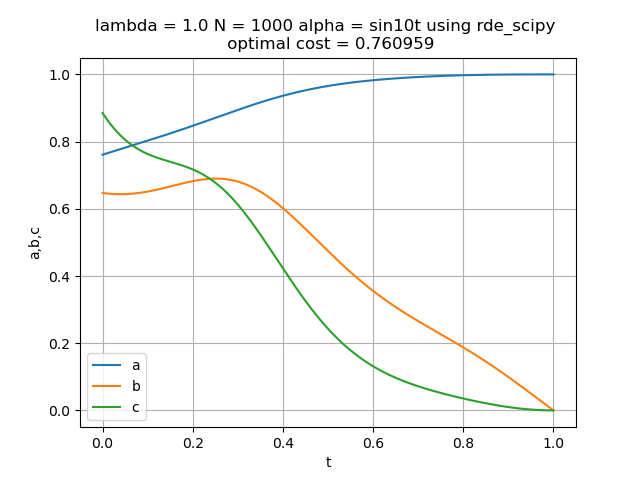
\includegraphics[width=\linewidth]{rde_scipy_l1_alphasin.png}
		\caption{RDE LSODE}
	\end{minipage}
	\hfill
	\begin{minipage}{0.3\textwidth}
		\centering
		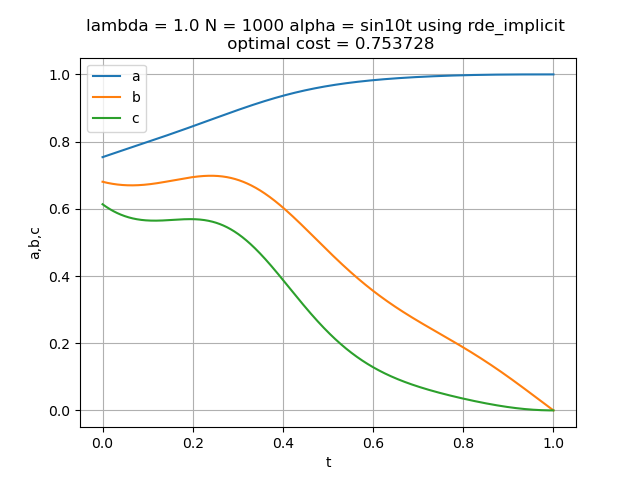
\includegraphics[width=\linewidth]{rde_implicit_l1_alphasin.png}
		\caption{RDE Implicit}
	\end{minipage}
	\hfill
	\begin{minipage}{0.3\textwidth}
		\centering
		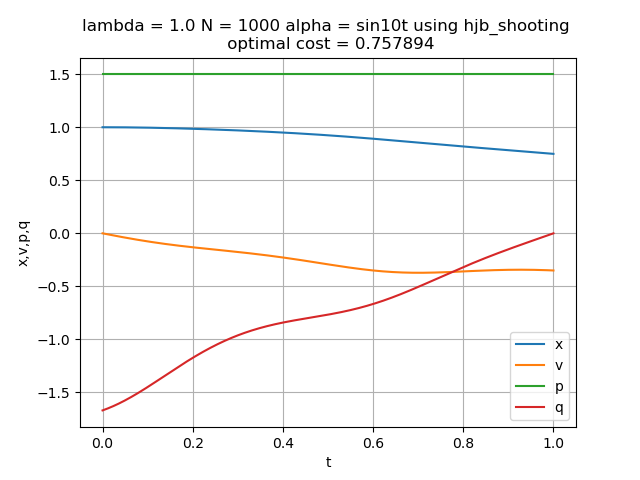
\includegraphics[width=\linewidth]{hjb_shooting_l1_alphasin.png}
		\caption{HJB Shooting}
	\end{minipage}
	\caption{$\lambda = 1, \alpha(t) = \sin(10 t)$}
\end{figure}

\begin{figure}[H]
	\centering
	\begin{minipage}{0.3\textwidth}
		\centering
		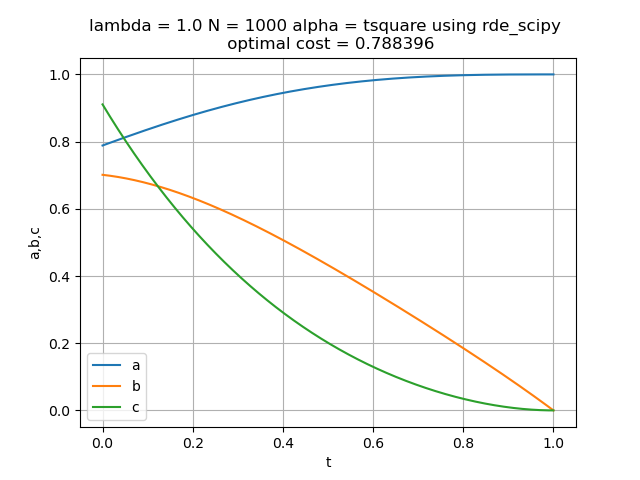
\includegraphics[width=\linewidth]{rde_scipy_l1_alphat2.png}
		\caption{RDE LSODE}
	\end{minipage}
	\hfill
	\begin{minipage}{0.3\textwidth}
		\centering
		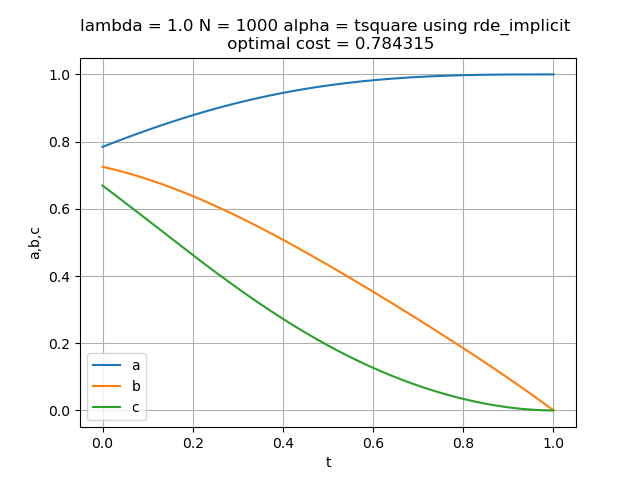
\includegraphics[width=\linewidth]{rde_implicit_l1_alphat2.png}
		\caption{RDE Implicit}
	\end{minipage}
	\hfill
	\begin{minipage}{0.3\textwidth}
		\centering
		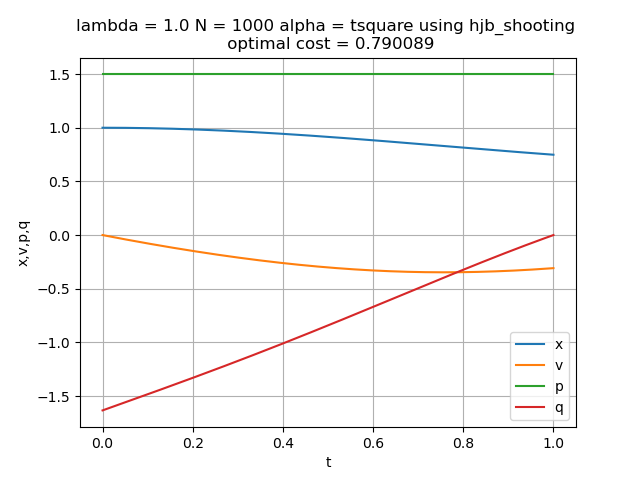
\includegraphics[width=\linewidth]{hjb_shooting_l1_alphat2.png}
		\caption{HJB Shooting}
	\end{minipage}
	\caption{$\lambda = 1, \alpha(t) = t^2$}
\end{figure}

\subsubsection{$\lambda = 0.1$}

When $\lambda = 0.1$, it is \textit{very easy} to control $x$ by $u$ since it does not induce too much cost, the optimal cost is lower. However, \textbf{RDE LSODE} failed to produce the result.

\begin{figure}[H]
	\centering
	\begin{minipage}{0.45\textwidth}
		\centering
		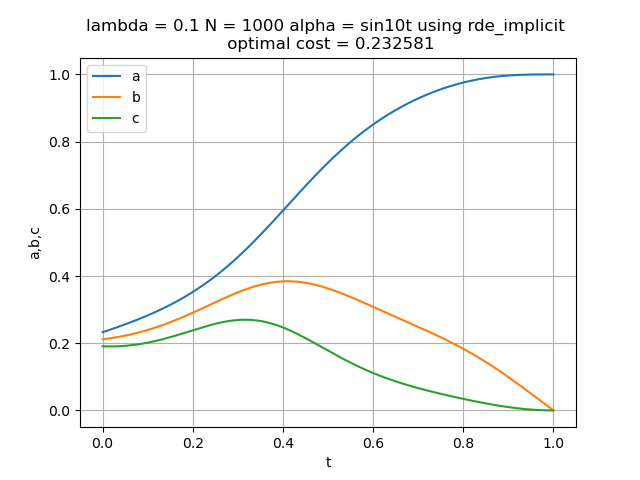
\includegraphics[width=\linewidth]{rde_implicit_l01_alphasin.png}
		\caption{RDE Implicit}
	\end{minipage}
	\hfill
	\begin{minipage}{0.45\textwidth}
		\centering
		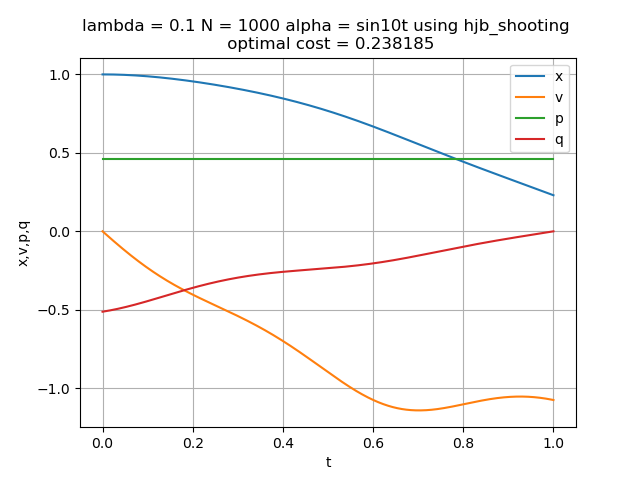
\includegraphics[width=\linewidth]{hjb_shooting_l01_alphasin.png}
		\caption{HJB Shooting}
	\end{minipage}
	\caption{$\lambda = 0.1, \alpha(t) = \sin(10 t)$}
\end{figure}

\subsubsection{$\lambda = 10$}

When $\lambda = 10$, it is \textit{very hard} to control $x$ by $u$ since it does induce a lot of cost for a positive value of $u$, the optimal cost is closed to $1$ which is the case when $u(t) = 0$. all three methods were able to produce a result for optimal control.

\begin{figure}[H]
	\centering
	\begin{minipage}{0.3\textwidth}
		\centering
		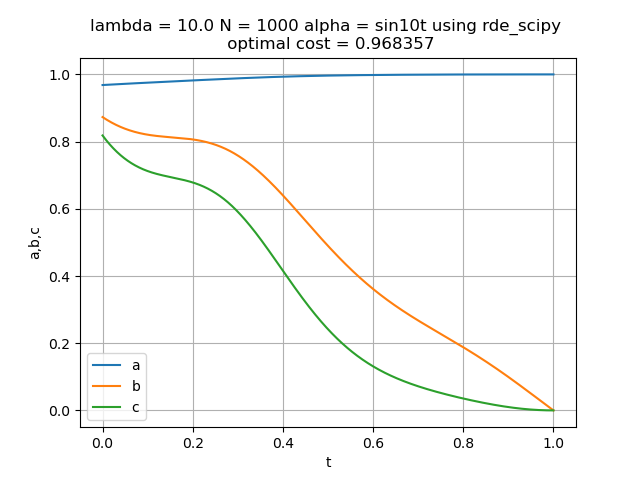
\includegraphics[width=\linewidth]{rde_scipy_l10_alphasin.png}
		\caption{RDE LSODE}
	\end{minipage}
	\hfill
	\begin{minipage}{0.3\textwidth}
		\centering
		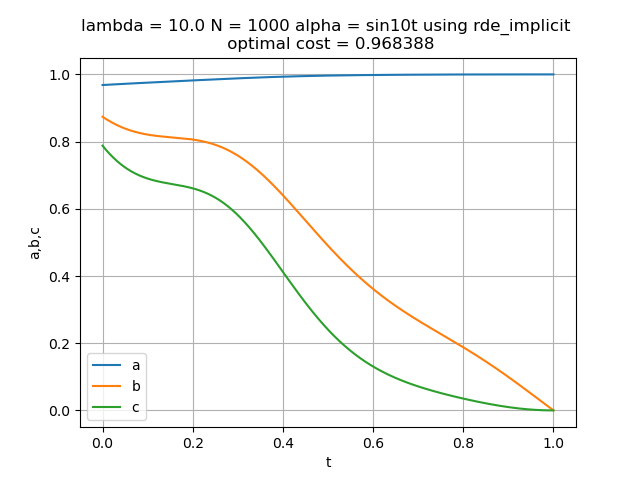
\includegraphics[width=\linewidth]{rde_implicit_l10_alphasin.png}
		\caption{RDE Implicit}
	\end{minipage}
	\hfill
	\begin{minipage}{0.3\textwidth}
		\centering
		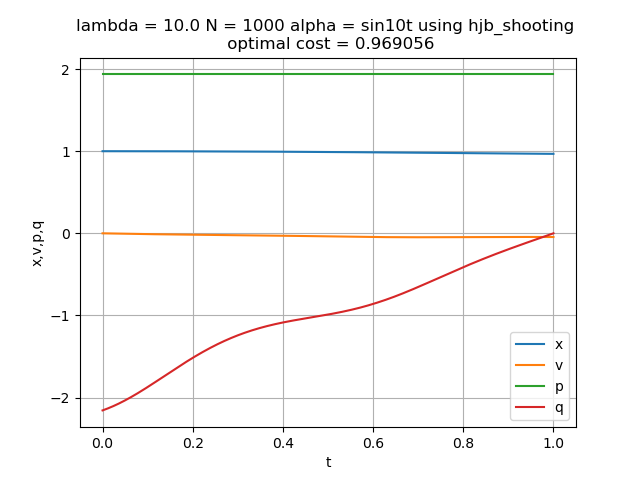
\includegraphics[width=\linewidth]{hjb_shooting_l10_alphasin.png}
		\caption{HJB Shooting}
	\end{minipage}
	\caption{$\lambda = 10, \alpha(t) = \sin(10 t)$}
\end{figure}

\begin{figure}[H]
	\centering
	\begin{minipage}{0.3\textwidth}
		\centering
		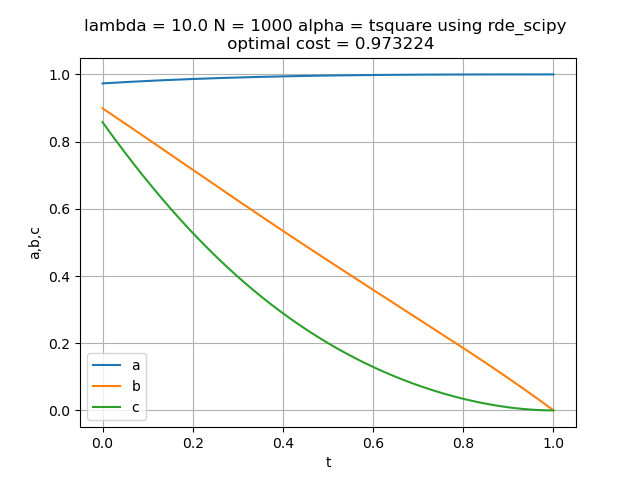
\includegraphics[width=\linewidth]{rde_scipy_l10_alphat2.png}
		\caption{RDE LSODE}
	\end{minipage}
	\hfill
	\begin{minipage}{0.3\textwidth}
		\centering
		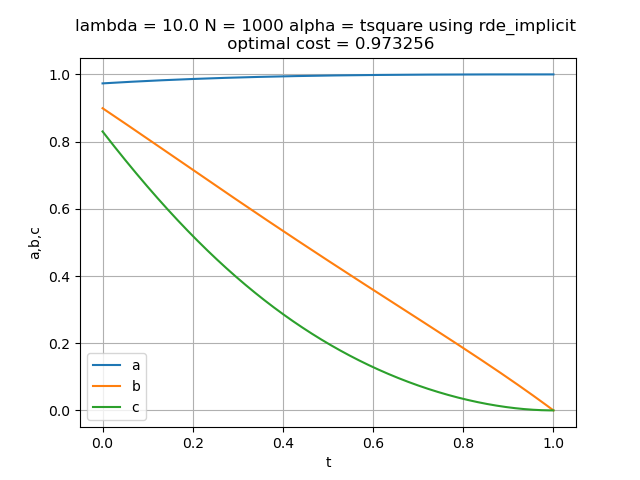
\includegraphics[width=\linewidth]{rde_implicit_l10_alphat2.png}
		\caption{RDE Implicit}
	\end{minipage}
	\hfill
	\begin{minipage}{0.3\textwidth}
		\centering
		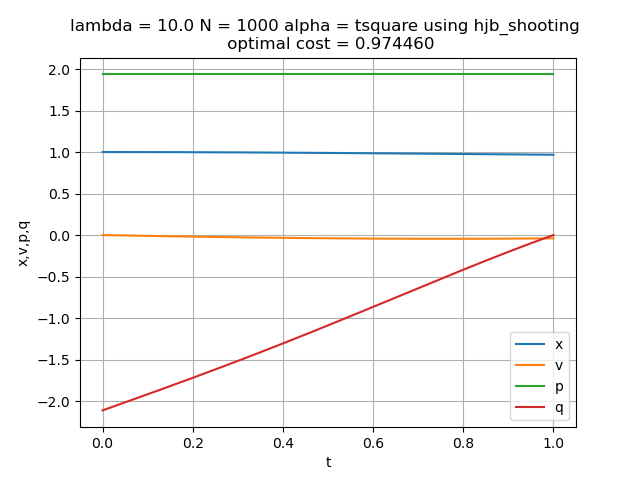
\includegraphics[width=\linewidth]{hjb_shooting_l10_alphat2.png}
		\caption{HJB Shooting}
	\end{minipage}
	\caption{$\lambda = 10, \alpha(t) =t^2$}
\end{figure}

\pagebreak

\section{CODE}

\lstinputlisting[language=python]{code.py}


